\section{Fundamentals}

The following section provides clarity to concepts and details necessary to understand the paper.

\subsection{Entity Component System}
An Entity Component System (ECS) is a software architecture pattern commonly used in game development and simulations to manage objects \cite{RomeoPHD}. All ECS's contain three parts:
\begin{enumerate}
    \item \textbf{Entity:} An entity is an object that serves as a unique identifier. Entities themselves carry no data or have inherent behaviors. They are IDs that link together components
    \item \textbf{Component:} Components are data containers that store attributes or properties for an entity. Each component typically holds data relevant to one aspect of an entity like position, or health. Unlike entities, components do carry data but do not have any inherent behaviors.
    \item \textbf{System:} A system contains the logic that operates on entities. A system processes entities that possess groups of components requested by the system. For example, a rendering system might process groups of entities that contain both a position and a texture component. 
\end{enumerate}

\subsubsection{ECS Characteristics}
The ECS pattern is classified as an architectural design pattern under Data-Oriented Design (DOD)\cite{RomeoPHD}. DOD is a programming paradigm that emphasizes efficient organization and access of data. Unlike Object-Oriented Design (OOP), which focuses on behavior encapsulation, DOD focuses on data storage and data access. It also includes concepts and techniques to maximize performance using specific memory access patterns and CPU cache utilization techniques.

The reasoning why ECS is classified under DOD is mainly due to two reasons: separation of concerns and composition over inheritance.

\begin{enumerate}
    \item \textbf{Separation of Concerns:} Separation of Concerns is a design principle that aims to divide a program into distinct sections able to operate independently. An ECS provides this distinction. For example an ECS separates data from behavior by having components from systems separate, respectively. This leads to more modular and maintainable code.
    \item \textbf{Composition over Inheritance: }Composition over Inheritance is a design principle that favors composing objects out of existing, reusable parts instead of over inheritance via some class hierarchy. Entities in an ECS are composed of multiple components, allowing for flexible combinations of complex objects without deep inheritance hierarchies. 
\end{enumerate}

\subsubsection{Written Example:}
To get a feeling for what an ECS is capable of, let's imagine a simple game with moving characters. We need to think of how to structure the ECS. 

In order for our character to move on the screen, they are going to need to know about their position and where they are going. The character also needs to be somehow rendered to the screen so there needs to be data about the texture. We can take these ideas and consider the scenario we pick the following components:

\begin{itemize}
    \item \texttt{PositionComponent: }The X,Y position of where the character is.
    \item \texttt{VectorComponent: }The direction of where our character is facing. Is X,Y
    \item \texttt{TextureComponent: }Stores the texture of the player character.
\end{itemize}

Even though we decided on the three components above, this does not indicate this was our only choice. There is nothing stopping us from making a larger component, call it \texttt{PlayerComponent} that contains the position, vector, and texture component data all put into one object. The motivation behind dividing these into the smallest pieces possible is that these segments of data can be targeted more precisely by related systems. 

An example of this is say later down the line, we decide to implement static entities in our game like walls or a floor. If we only had \texttt{PlayerComponent}, we would have to create another component to store the position and textures of this new entity kind. We would also need to duplicate our rendering efforts and write a new system specifically for static entities since both do not share a texture component type. This is not so great. 

But if we we use the three components listed above, the renderer could be re-used, stay the same, and no new component definitions are necessary. The moving character would have the three defined components and the static entities would have all except \texttt{VectorComponent}, since static entities do not move.

Now with the data in order, we need to consider what systems are required for getting the character to move. It makes most sense for there to be two systems:

\begin{itemize}
    \item \texttt{MovementSystem: }Requests the \texttt{VectorComponent} and reads I/O to see which arrow key is being pressed. Based on the key, update the component to point that direction.
    \item \texttt{RenderSystem: }Requests the \texttt{PositionComponent} and \texttt{TextureComponent}. It reads the position of all the entities and places the texture at that location. 
\end{itemize}

The \texttt{MovementSystem} would only look for entities that have the \texttt{VectorComponent}, and because of this our change to adding static entities to the ECS did not change any behavioral code. Since static entities will just use \texttt{PositionComponent} and \texttt{TextureComponent}, the \texttt{RenderSystem} also does not need to change.

\subsection{Ticks, Rates \& Concurrency}
Generally, in game development, a tick refers to the count of times at which a game has updated its state and processed all game logic once \cite{Gregory_2018}. A easier to understand way is to look at the code below: 

\begin{figure}[H]
    \begin{lstlisting}[
        language=Java,
        numbers=none
    ]
    int main() {
        // Do initialization steps for simulation here
        int tick = 0;
        while(gameRunning) {
            doGameLoop();
            tick++;
        }
        // Do cleanup steps for simulation here
        return 0;
    }
\end{lstlisting}
    \caption{Tick Example}
    \label{code:naive_ecs_data}
\end{figure}

\subsubsection{Ticks}

The code above shows that for each time the program processes one game loop, the tick goes up. Ticks are used as internal timestamps in engines most of the time, but are useless when it comes to actually measuring time between ticks. These timestamps are used generally for testing if data is stale or not, and other internal processes. 

\subsubsection{Tickrate}

The tick-rate is the frequency at which these ticks occur, usually measured in ticks per second (Hz) \ref{Gregory_2018}. It determines how often a simulation is capable of updating its state and process all logic. Higher tick-rates mean a stronger, more performant engine. 

A tick-rate of 60Hz, for example, means that the simulation updates 60 times per second. This does not necessarily equate to more frames per second. A simulation, for example, may be able to achieve a tick-rate of 60Hz but only actually render a new game frame every 3 ticks, so at 20Hz. This would mean this simulation would run at a tick-rate of 60Hz but have 20 frames per second. 

\subsubsection{Serialization Points}
A serialization point is a concurrency concept that specifies there exists a specific point in a program where operations are ordered or synchronized. A serialization point ensures execution correctness since it provides a data guarantee of being synchronized and consistent \cite{Herlihy_2021b}.

The key concepts to know about serialization points are:
\begin{enumerate}
    \item \textbf{Consistency:} Serialization points main data integrity by ensuring shared resources are accessed in a manner preventing data corruption.
    \item \textbf{Ordering:} Serialization points enforce order of operations.
\end{enumerate}

It turns out that the step of incrementing the tick counter can be considered a serialization point. Because of this, the GECS library uses the tick counter to continue data integrity in a manner such as shown below:


\begin{figure}[H]
    \begin{lstlisting}[
        language=Java,
        numbers=none
    ]
    int main() {
        // Do initialization steps for simulation here
        int tick = 0;
        while(gameRunning) {
            /* In Main Thread, Prepare For Loop */    

            /* Magic Done Here, Doing Many Threads */
            doGameLoopConcurrently();
            waitForGameLoop();

            /* Serialization Point Reached! In Main Thread */
            tick++;

            /* Do Cleanup Here */
        }
        // Do cleanup steps for simulation here
        return 0;
    }
\end{lstlisting}
    \caption{Tick Example}
    \label{code:naive_ecs_data}
\end{figure}

The above code is generally how most game engines work, with the same set of phases: preparation, execution, cleanup. Preparation and cleanup are both sequential routines, so they must only occur once the tick increases by 1 and the game loop has been processed once.

\subsubsection{The Wait Free Property}
Wait free in the context of concurrent programming refers to the behavior that each thread has some guarantee that it will complete its operation in a finite number of steps regardless of actions performed by other threads. Even if other threads are delayed by performing long operations, a model is wait-free if each thread is guaranteed to make progress within a bounded number of steps \cite{Herlihy_2021b}.

An example of what stops an algorithm from being wait-free, is waiting. If the algorithm requires any kind of synchronization in order to make progress, then that thread cannot guaranteed to make progress within a bounded number of steps.

\subsection{Types \& Archetypes}
In computer science, a type generally refers to a classification that specifies the kind of data an object or expression can hold. And sometimes the operations that can be performed on that data. Types are fundamental in that they give meaning to data and define structures. 

For an ECS, a type is used to encapsulate a component. An ECS type exists mainly to enforce a level of type safety inside the ECS. For example, suppose you are in a render system and you perform a request for a network component. This network component was obviously not included in the requirements list, and therefore this render system cannot access this component. This is the kind of type safety an ECS type gives \cite{SanderMertensECS}.

So in conclusion, an ECS type exists to encapsulate a component and to provide type enforcement either at compile time or runtime.

\subsubsection{Archetypes}
Archetypes are an extension of an ECS type introduced by Sander Mertens, the creator of the widely popular FLECS engine. An archetype, much like the ECS type, exist for type safety and component encapsulation. 

An archetype is a type used to encapsulate set of components. The GECS C Library introduced in this paper, uses archetypes for type safety around its concurrent model while also helping to keep components vectorized.

\subsection{Vectorization}
Vectorization is a process where operations are applied simultaneously to a set of values. This is typically done using specialized hardware instructions to improve performance, like SIMD. This technique is known to be extremely effective in scenarios containing large data-sets with repetitive calculations, such as physics, rendering, or even machine learning.  \cite{RomeoPHD}

To get the most out of vectorization, objects that are to have vectorized operations applied to them must be contiguous in memory. While it is possible to apply SIMD instructions over non-contiguous memory, you will be wasting memory bandwidth and there will be a drop in the programs cache efficiency. 

SIMD instruction sets typically include two very important instructions: load and store. These instructions are designed to move large contiguous blocks of memory into SIMD registers quickly and are very performant. This is the reason why when vectorization is mentioned in the paper, it is assumed that the memory is being prepared to be placed contiguously in memory. 

As mentioned earlier, it is possible to perform SIMD over non-contiguous memory using operations called scatter/gather operations but is not recommended. They work by gathering data from or scattering data to different locations. These operations are less efficient than load/store and incur overhead. Non-contiguous memory with SIMD also incurs more complex indexing strategies and complex indexing instructions associated with it. The concurrent model proposed attempts to avoid using these instructions at all costs. \cite{Kusswurm_2022}

\subsubsection{Key Vectorization Concepts}
\begin{enumerate}
    \item \textbf{Single Instruction, Multiple Data (SIMD):} SIMD is a type of parallel computing architecture where a single hardware instruction is designed to be applied to multiple data points simultaneously. Most modern GPUs and CPUs have some level of SIMD capabilities.
    \item \textbf{Vectorized Operations:} Operations that operate over an entire vector of data all at once rather than iterating through elements individually. A simple example of a vector operation could be adding two arrays of numbers together into a sum array, element-wise. If this algorithm is done in a single operation, then that operation is considered vectorized.
    \item \textbf{Data Parallelism:} Vectorization is a technique used to achieve data parallelism. This is where the same operation is performed on different pieces of distributed data concurrently. An example of something such as this is dividing a list of elements by a set of threads, and having the threads perform operations on the list. 
    \item \textbf{Task Parallelism:} This is in contrast to data parallelism, where threads are executed concurrently to perform distinct operations on the same or different set of data. An example of something such as this is concurrently adding the sum of different lists. The same summation task is done on each list, where each task is assigned to a different thread. 
\end{enumerate}

\subsubsection{Vectorization Benefits}
There are clear performance benefits to keeping data in an ECS vectorized. If an ECS is able to perform multiple operations on multiple data points in parallel, vectorization can significantly speed up computations. But vectorization also has other hidden benefits:
\begin{enumerate}
    \item \textbf{More Efficient Hardware Use:} Modern CPUs and GPUs designed for vectorized instructions can process multiple data points in a single clock cycle. This is not only good for performance, but takes better use of the hardware's capabilities.
    \item \textbf{Simple After Lots Of Thought:} Although vectorized code may be challenging to place and write, once it's developed vectorized code appears more concise and readable. This is because loops and other iterative strategies are no longer used, and explicit loops are unnecessary.
\end{enumerate}

\subsubsection{Challenges \& Negatives of Vectorization}
Although for how much vectorization can bring for performance gains and code readability, there are still many drawbacks to consider when vectorizing data.
\begin{enumerate}
    \item \textbf{Data Alignment:} A core issue for SIMD instructions is that data must be aligned to work efficiently, so extra care needs to be done around how data is organized. While SIMD can handle misaligned data, it will result in slower performance that's not worth the cost of using SIMD.
    \item \textbf{Introduced Complexity:} While vectorized code appears simpler, the implementation underneath SIMD can be exceedingly complex. To write good SIMD code, a good understanding of both the hardware you are designing with and the provided data structures are involved.
    \item \textbf{Portability:} Since SIMD are specialized CPU instructions, a lot of vectorized code depends on specific hardware features that are hard to generalize. 
\end{enumerate}

In conclusion about vectorization, the GECS C Library and the model proposed do not explicitly use SIMD instructions in any fashion. The objective of this library is to provide a platform that gives access to an already pre-vectorized set of requested ECS components for the library user to perform SIMD on, or to simply do some data parallelism on.

\subsection{Finite State Machine}
A Finite-State-Machine (FSM), also sometimes referred to as a finite automaton, is a computational model used to design programs. It consists of a finite number of states, some way to transition between those states, and a set of inputs that can be applied to to get to a different state. FSM's are used to generally model programs where the there are "states" the FSM can be in, and some inputs can change that state. 

A simple example of a finite state machine is imagine a man jumping. There are two known states the man can be in: jumping or not jumping. The transition between the states is how far off the ground he is. If the man's y coordinate is 0, then he is not jumping so he goes to the "not jumping" state. If the man's y coordinate is greater than 0, then he is jumping so he goes to the "jumping" state.

\begin{figure}[H]
    \centering
    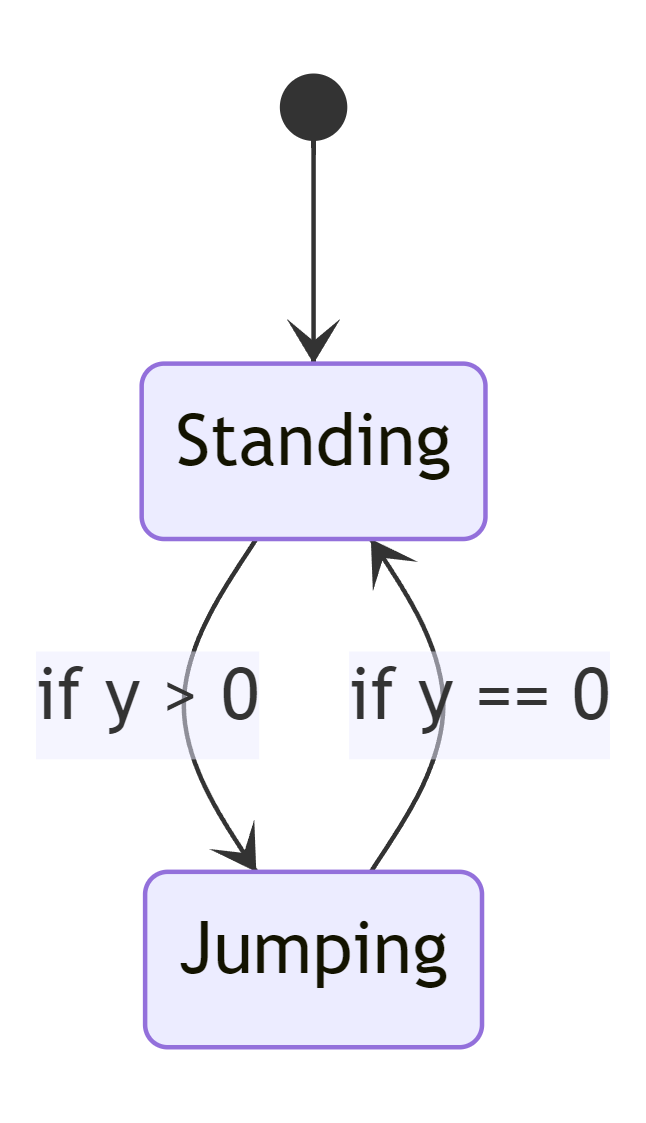
\includegraphics[width=0.25\linewidth]{resources/man_fsm_example.png}
    \caption{Man FSM Example}
    \label{fig:graph2}
\end{figure}

\subsubsection{Deterministic Finite Automaton}
A Deterministic Finite Automaton (DFA) is a type of finite state machine that uniquely defines for each state and input, exactly one transition to a new state. I argue that this is the type of state machine that the GECS Library uses. While it does not exactly have each state uniquely defined beforehand, all inputs for state transitions are valid, and therefore I would classify the FSM introduced with the concurrency model as a DFA.

\subsubsection{FSM Applications}
In the world of simulations, FSM's are fundamental because they provide closed systems with easy to understand behaviors that cause state transitions. The convenience of using FSM's in game programming can be expressed with how AI's are classically designed. Figure \ref{fig:soldier_fsm} below represents the behavior inhibited by a Non-Player Character (NC), one of the kinds of AI players interact with. Based on a couple of inputs: position, health, and the player, the NC changes it's state. This is all easily track-able when using a state machine.

\begin{figure}[H]
    \centering
    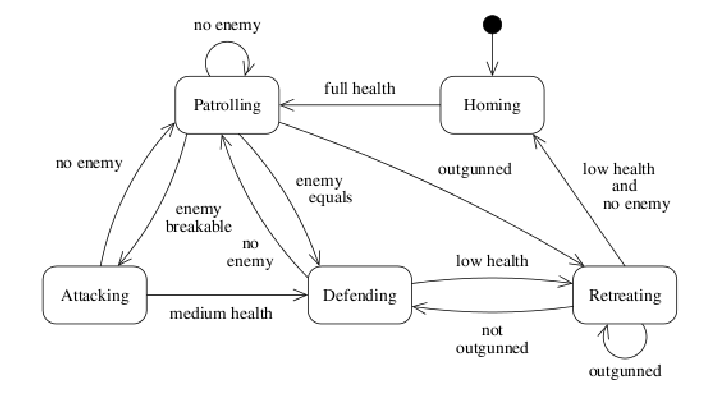
\includegraphics[width=0.8\linewidth]{resources/soldier_fsm.png}
    \caption{Example AI FSM \cite{FSM}}
    \label{fig:soldier_fsm}
\end{figure}